\documentclass[tikz]{standalone}
\usetikzlibrary{arrows.meta}
\begin{document}

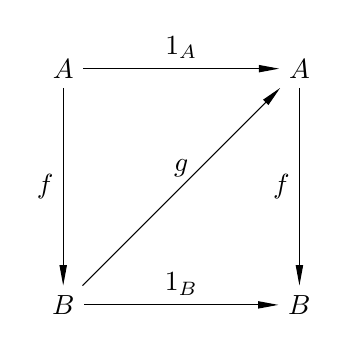
\begin{tikzpicture}[-latex, arrows={-Triangle[angle=20:5pt,scale=1.5]}]
	\node (A1) at (0,0) {\(A\)};
	\node (A2) at (3,0) {\(A\)};
	\node (B1) at (0,-3) {\(B\)};
	\node (B2) at (3,-3) {\(B\)};

	\draw (A1) to node [left] {\(f\)} (B1);
	\draw (A2) to node [left] {\(f\)} (B2);
	\draw (B1) to node [above] {\(g\)} (A2);

	\draw (A1) to node [above] {\(1_A\)} (A2);
	\draw (B1) to node [above] {\(1_B\)} (B2);
\end{tikzpicture}

\end{document}
